\section{Requirements and Preliminaries}
\label{sec:background}

% \begin{tcolorbox}
% \para{Goal} low-power bi-directional VLC.
% \para{Overview} backscattering lights using retro-reflector, modulate with LCD. 
% \para{Retro-reflector} principles, effects, properties 
% \para{LCD modulation} 
% \para{Principles} Use analog components as many as possible (to avoid ADCs) and avoid complicated digital signal processing on the mobile end. Also, design amplifiers that work at an almost-cut-off state to save energy cost. \todo{what does this sentence mean?}
% \end{tcolorbox}


Our goal is to design a bi-directional VLC system that runs on battery-free devices like smartphones and sensor nodes. The system features an LED and a mobile device. One closed-loop communication paradigm of the system is as follows. The LED sends a packet carried on the white light it emits modulated to $1MHz$ (downlink). The \vitag\ senses the transmission and wakes up. Upon successfully receiving and demodulating the packet, the \vitag\ sends a packet back to the LED (uplink). The LED is slightly modified so as to integrate the receiver in as shown in Fig.~\ref{fig:system}.

In sending the packet, instead of generating the signal using power-consuming LEDs or other communication channels such as infrared or ultraviolet carriers, we adopt the modulating retro-reflector framework, with the combination of an LCD and a retro-reflector. Driving the LCD costs only $400-\mu W$ energy. In addition, a \vitag\ passively sends signals, thus the power consumption of which can be maintained at a low level. 

%with the help from other energy saving components. Finally,  The receiver detects any signals sent by the \vitag, and decodes the bits against noises and interferences.

In the rest of the paper, we describe the design of \retro\ that consists of a modified off-the-shelf white LED and a \vitag\ in more details.

%\p{We need a system architecture figure here}

% Our goal is to design primitives that enhance visible light communication capabilities on battery-free devices while preserving user privacy and security of both the transmitters and the receivers, with the omnipresence of readily available LEDs that serve as the lightening devices. The key challenge in achieving these is two-fold. First, devices running at visible light bands are power-intensive because of the broad bandwidth these bands can provide. Second, the noise caused by ambient signals on the visible light spectrum and the interference triggered by the the data transmitted by the system itself stays in the same band as what the receiver expects to receive at. To address these challenges, we use the following guiding principles: we use as many analog components and recycle as much energy as possible on the tag to enable the tag to transmit to the reader with a decent data rate. Also, we diminish the scattering area as much as possible by making use of directional backscattering materials of small Field of View (FoV). Such approaches, as we show in the rest of the paper, can provide an order of magnitude reduction in the power consumption of these communication primitives and in the scattering area of the signals on the backscattering channel.

% In the rest of this paper, we describe \vitag, our battery-free tag and show how it can enable backscatter communications with no battery and with a higher energy efficiency with respect to communication range than tags with LEDs on. We then describe \reader, our system that can be easily integrated onto commercial LED lights for transmitting data at no discernible flickers with dimming support and receiving with \hl{hhh dB} signal-to-interference-plus-noise-ratio (SINR). Finally, we show that our designs can be used to enable concurrent transmissions in a network of battery-free devices without the need for synchronization.



%\paragraph{Visible Light Communication} 
%Visible lights are electromagnetic waves that span frequencies roughly from 400 to 800 THz. For illumination, white LEDs are commonly used. The instantaneous On/Off feature turns LEDs into effective transmitters for visible light communication (VLC). Specifically, information bits can be embedded on the light by modulating the on/off state of the LED with on-off keying (OOK) or variable pulse-position modulation (VPPM) \cite{standard}. To receive such signals, while in some cases a cell phone camera or a digital camera will be sufficient \hl{need citations, ipsn14 and mobicom14}, photodiodes are generally used, because phone cameras can only achieve around 0.25MHz sampling rate~\cite{camera1} (in other words, low data rate), whereas photodiodes have generally higher bandwidth up to 0.5GHz~\cite{pdsheet}. Moreover, compared with a phone camera, the SNR of the photodiode is orders of magnitude higher at the same distance \hl{ipsn14}. 

%A typical way to generate white lights is to use a phosphor material to convert monochromatic lights from blue or ultraviolet to broad-band white lights, where the color of the monochromatic light depends on the band gap energy of the materials forming the p-n junction in the LED. 

%Visible lights bring safety advantages over communication waves of other common frequencies, because human eyes are much more sensitive to the strength of visible lights than the invisible TV, Wi-FI and RFID transmissions. With the LED dimming support~\cite{dimming}, a person can turn down the light if she feels of a too high brightness. In addition, radios waves at some certain frequencies are likely to hard human organs, especially to pregnant women and kids~\cite{rfidharm}, while the visible light are not.

%There are two primary ways of producing white LEDs. One is to use individual LEDs that emit three primary colors --- red, green, and blue --- and then mix all the colors to form white light~\cite{ledprin1}. The other is to use a phosphor material to convert monochromatic light from a blue or UV LED to broad-spectrum white light, much in the same way a fluorescent light bulb works~\cite{ledprin2}. In general, the wavelength of the light emitted, and thus its color, depends on the band gap energy of the materials forming the p-n junction. In materials used for LEDs, the electrons and holes recombine by a radiative transition, which produces optical emission, because there are direct band gap with energies corresponding to near-infrared, visible, or near-ultraviolet light. 





\paragraph{Retro-reflector} 
Retro-reflector is a device that operates by returning light back to the light source along the same light direction with a minimum of scattering~\cite{rr}. Retro-reflectors are widely used on road signs, bicycles, and clothing for road safety. From a microscopic view, a retro-reflector is composed of cells, each of which is a corner cube as shown in Fig.~\ref{fig:retrolcd} (e). When a light beam hits one of the cells, the light is turned around via two adjacent reflections. 



\paragraph{Modulating Retro-reflector}
Modulating retro-reflector (MRR)~\cite{mrr} consists of a retro-reflector and a modulator for optical communications. An MRR operates as a passive sources which transmits bits by varying the intensity of the reflected light beam. MRR is widely used in free space communication where the other side is a laser. Existing MRR systems~\cite{expensive,expensive2} is usually of a large size, and modulation is commonly achieved with a high-end electroabsorption modulator altering the absorption spectrum by applying an electric field. Consequently, such setting is ill-suited for our scenarios which require a low-cost solution.
\p{Need double check. It is really hard to understand the existing MRR solutions. Cannot find much material.}

LCD is \todo{polarized glass + liquid, liquid can polarize incoming light, } LCDs use the light properties of liquid crystals that are controlled by the voltage added on them. When the LCD is on, the incoming light is able to pass the LCD and hit the retro-reflector; When the LCD is off, the incoming light is rejected by the LCD. Therefore, LCDs can be used as modulators for MRRs. 
%However, one disadvantage of LCDs are their low refresh rate, e.g., 60 or 75 Hz, which is too low for data communication. Fortunately, we find \textit{LCD shutters} with much higher refresh rate (up to 1KHz \hl{cite}). Fig.~\ref{fig:retrolcd} shows the basic principle of a retro-reflector with an LCD coverage.
\begin{figure}[th]
   \centering
   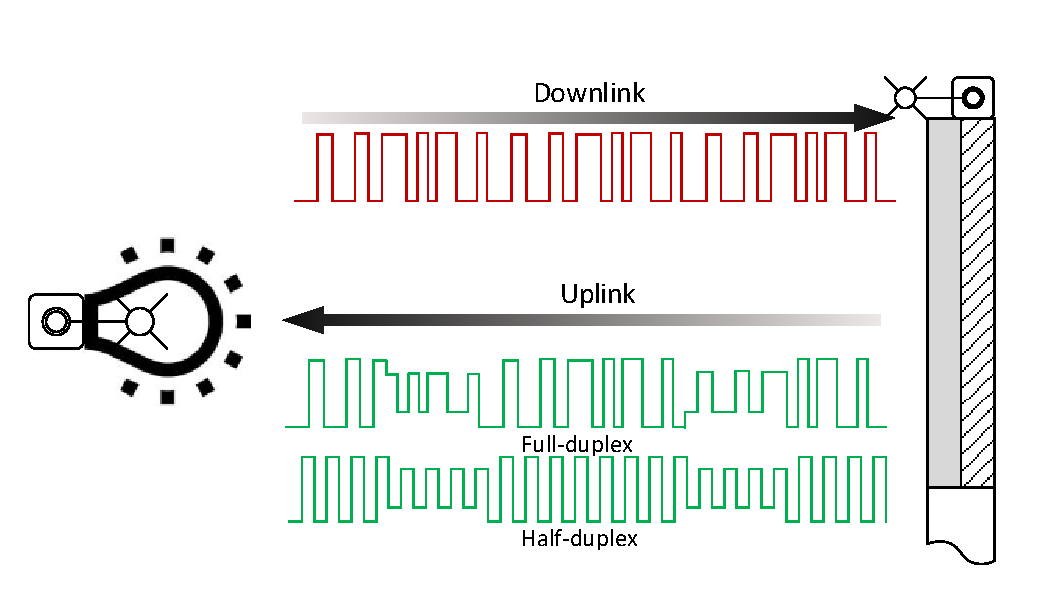
\includegraphics[width=0.8\columnwidth]{link.pdf}
   \caption{Downlink and uplink.}
   \label{fig:link}
   \vskip -3mm
\end{figure}

\figref{fig:link} illustrates the modulated uplink lights using LCD. We notice that the commercially off-the-shelf LCDs are of low refreshing rate. Therefore, the symbol length is relatively much longer than the carrier waveform.


\begin{figure*}[!t]
\vskip -0.1in
\centering
{\footnotesize
\begin{tabular}{ccccc}
\epsfig{file=../illustrations/mrr1.eps, height=0.2\columnwidth} &
\epsfig{file=../illustrations/mrr2.eps, height=0.2\columnwidth} & 
\epsfig{file=../illustrations/mrr3.eps, height=0.2\columnwidth} & 
\epsfig{file=../illustrations/mrr4.eps, height=0.2\columnwidth} &
\epsfig{file=../illustrations/retroreflector.eps, height=0.2\columnwidth} \\
{(a) TX $45\degree$, RX $45\degree$} & 
{(b) TX $45\degree$, RX $135\degree$} & 
{(c) TX $45\degree$, RX $90\degree$} & 
{(d) TX $90\degree$, RX $90\degree$} &
{(e) Ideal Retro-reflector} \\
\end{tabular}
}
\vskip -0.1in
\caption{\footnotesize{\bf Illustration of the Retro-reflector.} (a) When the LED (TX) is at $45\degree$ arrival of incidence, and the camera (RX) is at $45\degree$, the retro-reflector area (on the right) is bright, the mirror area (in the middle) is dark, and the paper area (on the left) is dark. (b) When the LED is at $45\degree$, and the camera is at $135\degree$, the mirror area is bright, while the retro-reflector and the paper areas are dark. (c) When the LED is at $45\degree$, and the camera is at $90\degree$, the retro-reflector and the mirror areas are dark, while the paper area is slightly bright due to diffused reflections. (d) When the LED is at $90\degree$, and the camera is at $90\degree$, both the retro-reflector and mirror areas are bright. (e) depicts an ideal retro-reflector and how it responds to incoming lights. Our actual retro-reflector has a scattering angle as small as $5\degree$}
\label{fig:retrolcd}
\vspace{-1em}
\end{figure*}




